\documentclass[12pt, a4paper]{report}

\usepackage[T1]{fontenc}
\usepackage[utf8]{inputenc}
\usepackage[english]{babel}
\usepackage[top=1in, bottom=1in, left=1.1in, right=1.1in]{geometry}

% math packages
\usepackage{amsmath}
\usepackage{amssymb}
\usepackage{hyperref}
% graphics and tables
\usepackage{graphicx}
\usepackage{booktabs}

% code and algo
\usepackage{xcolor}
\usepackage{listings}
\usepackage{algorithm2e}
\usepackage{amsthm}
\newtheorem{definition}{Definition}

\renewcommand{\lstlistingname}{File}

\graphicspath{{attachments/}}
\RestyleAlgo{boxed}
\hypersetup{
    colorlinks=true,
    linkcolor=blue,
    filecolor=magenta,
    urlcolor=cyan,
    citecolor=green
}

% code block
\lstset{
    basicstyle=\ttfamily\small,
    keywordstyle=\color{blue}\bfseries,
    stringstyle=\color{red},
    commentstyle=\color{green!50!black},
    numbers=left,
    numberstyle=\ttfamily\scriptsize\color{gray}, numbersep=8pt,
    xleftmargin=15pt,
    frame=single,
    framexleftmargin=15pt,
    showstringspaces=false,
    breaklines=true,
    breakatwhitespace=false,
    keepspaces=true,
    columns=fullflexible,
    frame=single,
    framerule=1pt,
    framesep=5pt,
    backgroundcolor=\color{gray!10},
    tabsize=2
}

% \lstdefinelanguage{CSS}{
%   keywords={
%     color, background, margin, padding, border, display,
%     flex, justify-content, align-items,
%     height, width, font-family
%   },
%   sensitive=true,
%   morecomment=[s]{/*}{*/},
%   morestring=[b]",
%   morestring=[b]'
% }

% \lstdefinelanguage{JavaScript}{
%   keywords={let,const,var,function,return,if,else,for,while,break,continue,new,this},
%   keywordstyle=\color{blue}\bfseries,
%   sensitive=true,
%   morecomment=[l]{//},
%   morecomment=[s]{/*}{*/},
%   commentstyle=\color{green!50!black},
%   morestring=[b]",
%   morestring=[b]',
%   stringstyle=\color{red}
% }

\begin{document}
    \title{\huge Advanced Web Technologies \\ Lab Practical File}
    \author{
        \textbf{Sree Saicharan Vadapalli} \\
        Information Technology Department \\
        ET23BTIT133 \\
    }
    \date{February 18, 2026}
    \maketitle
    \newpage

    \tableofcontents
    \newpage

    \renewcommand{\chaptername}{Practical}

    \chapter{Registration Form with Client-Side Validation}

    \section{Problem Statement}
    Create a registration form and apply CSS and perform at least five JavaScript validations.

    \section{Implementation}
    Please note that this practical was implemented using a single HTML file with inline CSS and JavaScript.
    \begin{lstlisting}[caption={\texttt{index.html}}]
    <!DOCTYPE html>
    <html lang="en">
    <head>
    <meta charset="UTF-8">
    <meta name="viewport" content="width=device-width, initial-scale=1.0">
    <title>registration form</title>

    <style>
        body {
            font-family: Fira Sans, sans-serif;
            background: #282828;
            display: flex;
            justify-content: center;
            align-items: center;
            height: 100vh;
        }

        .container {
            background: #ffffff;
            padding: 30px;
            border-radius: 8px;
            width: 350px;
            box-shadow: 0 0 20px rgba(255,255,255,0.08);
        }

        h2 {
            text-align: center;
            margin-bottom: 20px;
        }

        input {
            width: 100%;
            padding: 8px;
            margin: 8px 0;
            border-radius: 4px;
            border: 1px solid #ccc;
        }

        .error {
            color: #ff4d4d;
            font-size: 12px;
        }

        button {
            width: 100%;
            padding: 10px;
            background-color: #4e73df;
            color: white;
            border: none;
            border-radius: 4px;
            cursor: pointer;
        }

        button:hover {
            background-color: #2e59d9;
        }
    </style>
    </head>

    <body>

    <div class="container">
        <h2>Registration Form</h2>

        <form id="registrationForm">
            <input type="text" id="name" placeholder="full name">
            <div class="error" id="nameError"></div>

            <input type="text" id="email" placeholder="email">
            <div class="error" id="emailError"></div>

            <input type="password" id="password" placeholder="password">
            <div class="error" id="passwordError"></div>

            <input type="password" id="confirmPassword" placeholder="confirm password">
            <div class="error" id="confirmPasswordError"></div>

            <input type="text" id="phone" placeholder="phone number">
            <div class="error" id="phoneError"></div>

            <input type="number" id="age" placeholder="age">
            <div class="error" id="ageError"></div>

            <button type="submit">register</button>
        </form>
    </div>

    <script>
    document.getElementById("registrationForm").addEventListener("submit", function(event) {

        event.preventDefault();

        let isValid = true;

        let name = document.getElementById("name").value.trim();
        let email = document.getElementById("email").value.trim();
        let password = document.getElementById("password").value;
        let confirmPassword = document.getElementById("confirmPassword").value;
        let phone = document.getElementById("phone").value.trim();
        let age = document.getElementById("age").value;

        document.querySelectorAll(".error").forEach(el => el.textContent = "");

        // name val
        let namePattern = /^[A-Za-z ]+$/;
        if (!namePattern.test(name)) {
            document.getElementById("nameError").textContent =
                "name should contain only letters and spaces";
            isValid = false;
        }

        //  email val
        let emailPattern = /^[^ ]+@[^ ]+\.[a-z]{2,3}$/;
        if (!emailPattern.test(email)) {
            document.getElementById("emailError").textContent =
                "enter a valid email address";
            isValid = false;
        }

        // password length val
        if (password.length < 8) {
            document.getElementById("passwordError").textContent =
                "password must be at least 8 characters";
            isValid = false;
        }

        // password strength val
        let strongPasswordPattern =
            /^(?=.*[a-z])(?=.*[A-Z])(?=.*\d)(?=.*[@$!%*?&])/;
        if (!strongPasswordPattern.test(password)) {
            document.getElementById("passwordError").textContent =
                "password must include uppercase lowercase number and special character";
            isValid = false;
        }

        // password match val
        if (password !== confirmPassword) {
            document.getElementById("confirmPasswordError").textContent =
                "passwords do not match";
            isValid = false;
        }

        // phone number val
        let phonePattern = /^[0-9]{10}$/;
        if (!phonePattern.test(phone)) {
            document.getElementById("phoneError").textContent =
                "phone number must be 10 digits";
            isValid = false;
        }

        // age val
        if (age < 18) {
            document.getElementById("ageError").textContent =
                "you must be at least 18 years old";
            isValid = false;
        }

        if (isValid) {
            alert("registration successful");
        }
    });
    </script>
    </body>
    </html>
    \end{lstlisting}
    \newpage

    \section{Results}
    \begin{figure}[h]
    \centering
    \fbox{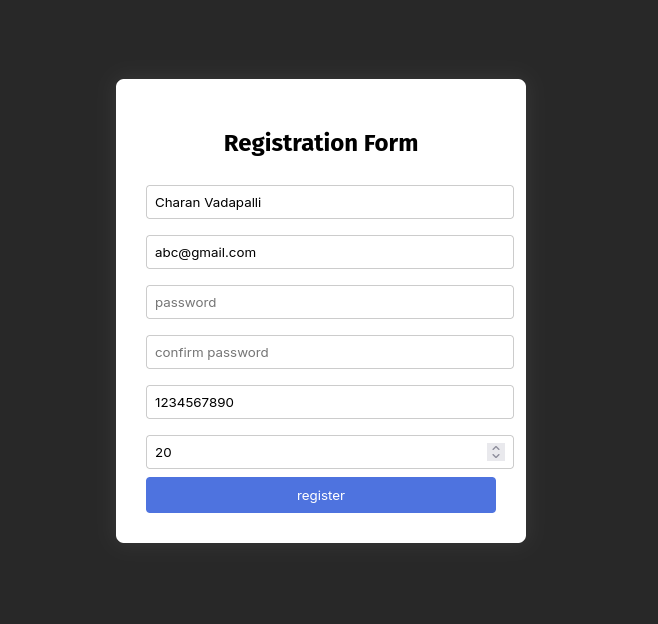
\includegraphics[width=0.7\textwidth]{registration-form.png}}
    \caption{Registration Form Output}
    \end{figure}

    \section{Conclusion}
    In this practical, a registration form was successfully implemented using basic HTML, CSS and JavaScript. The form includes validation for email, password, confirm password, phone number, and age. The form was tested using various inputs and was found to be functional and user-friendly.
    \\\\
    \vspace{1em}
    \begin{center}
        \rule{0.8\textwidth}{0.6pt}
    \end{center}
    \vspace{1em}

    \chapter{Number Guessing Game}

    \section{Problem Statement}
    Create a simple guess for the number type game. It should choose a random number between 1 and 100, then challenge the player to guess the number in 10 turns. After each turn the player should be told if they are right or wrong, and if they are wrong, whether the guess was too low or too high. It should also tell the player what numbers they previously guessed. The game will end once the player guesses correctly, or once they run out of turns. When the game ends, the player should be given an option to start playing again.

    \section{Implementation}

    \begin{lstlisting}[caption={\texttt{index.html}}]
    <!DOCTYPE html>
    <html>
    <head>
        <link rel="stylesheet" href="style.css">
    </head>

    <body>

        <form onsubmit="event.preventDefault(); deep();">
            Take a guess:
            <input type="text" id="guess">
            <input type="button" value="Submit" onclick="deep()">
        </form>

        <div class="completed">Game Is Completed!</div>
        <div id="guesstell"></div>
        <div id="write"></div>
        <div id="current"></div>

        <button onclick="again()" class="playagain">
            Play Again
        </button>

        <script src="script.js"></script>
    </body>
    </html>
    \end{lstlisting}

    \begin{lstlisting}[caption={\texttt{style.css}}]
    body {
        margin: 0;
        font-family: "Fira Sans", sans-serif;
        background: #282828;
        color: #ebdbb2;
        display: flex;
        justify-content: center;
        align-items: center;
        height: 100vh;
    }

    form {
        background: #3c3836;
        padding: 20px;
        border: 1px solid #504945;
    }

    input, button {
        padding: 6px;
        margin: 6px 0;
        background: #282828;
        color: #ebdbb2;
        border: 1px solid #504945;
    }

    button {
        background: #fabd2f;
        color: #282828;
    }
    \end{lstlisting}

    \begin{lstlisting}[caption={\texttt{script.js}}]
    let trial = 0;
    let random;
    let guesses = [];

    // start the game immediately
    again();

    function again() {
        trial = 0;
        guesses = [];

        // updated range: 1 to 100
        random = Math.floor(Math.random() * 100) + 1;
        console.log("Secret Number:", random);

        // reset ui
        document.querySelector(".completed").style.display = "none";
        document.querySelector(".playagain").style.display = "none";

        document.getElementById("write").innerHTML = "Start guessing...";
        document.getElementById("guesstell").innerHTML = "";
        document.getElementById("current").innerHTML = "";
        document.getElementById("guess").value = "";
    }

    function deep() {
        const inputField = document.getElementById("guess");
        let usernumber = Number(inputField.value);

        // basic validation
        if (!usernumber || usernumber < 1 || usernumber > 100) {
            alert("Enter a valid number between 1 and 100!");
            return;
        }

        // check win condition
        if (usernumber === random) {
            document.getElementById("guesstell").innerHTML =
                "The number was " + random;

            document.querySelector(".playagain").style.display = "block";
            return;
        }

        // wrong guess logic
        trial++;
        guesses.push(usernumber);

        inputField.value = "";
        inputField.focus();

        if (usernumber > random) {
            document.getElementById("guesstell").innerHTML =
                "High! Try lower.";
        } else {
            document.getElementById("guesstell").innerHTML =
                "Low! Try higher.";
        }

        document.getElementById("write").innerHTML =
            "Attempts used: " + trial + " / 10";

        document.getElementById("current").innerHTML =
            "History: " + guesses.join(", ");

        // check lose condition
        if (trial >= 10) {
            endGame();
        }
    }

    function endGame() {
        document.getElementById("write").innerHTML =
            "Game Over! Better luck next time.";

        document.getElementById("guesstell").innerHTML =
            "The number was: " + random;

        document.querySelector(".completed").style.display = "block";
        document.querySelector(".playagain").style.display = "block";
    }
    \end{lstlisting}

    \section{Results}
    \begin{figure}[h]
    \centering
    \fbox{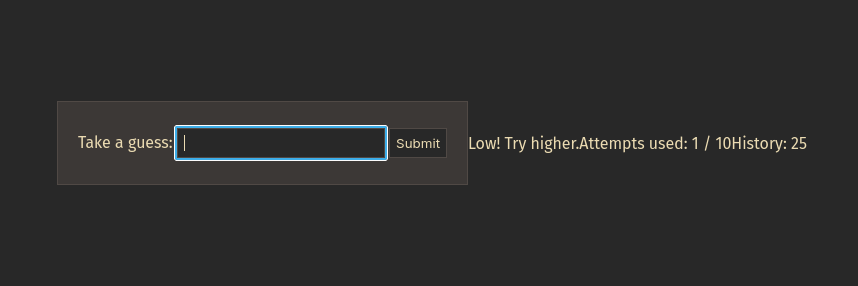
\includegraphics[width=0.7\textwidth]{number-game.png}}
    \caption{Number Guessing Game}
    \end{figure}

    \begin{figure}[h]
    \centering
    \fbox{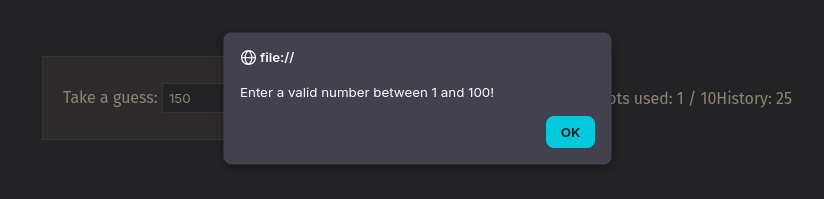
\includegraphics[width=0.7\textwidth]{number-game-invalid-input.png}}
    \caption{Invalid Input Scenario}
    \end{figure}
    \newpage

    \section{Conclusion}
    In this practical, a number guessing game was successfully developed using HTML, CSS and JavaScript. This practical is a basic demonstration of how to create a simple interactive web application using the above mentioned technologies. The program maintains internal states such as the current guess, the number of attempts, and the history of guesses and updates the DOM dynamically.
    \\\\
    \vspace{1em}
    \begin{center}
        \rule{0.8\textwidth}{0.6pt}
    \end{center}
    \vspace{1em}

    \chapter{Basic React Application}

    \section{Problem Statement}
    Create a Hello World Web Page using ReactJS.

    \section{Theory}
    ReactJS is a free and open-source front-end JavaScript library that aims to make building user interfaces based on components more seamless. It's maintained by Meta and a community of individual developers and companies.

    ReactJS is a declarative, component-based JavaScript library for building user interfaces, primarily for single-page applications. At its core, React models the UI as a function of state: given some state, the UI is deterministically rendered from it. Instead of manually manipulating the DOM (imperative approach), React uses a virtual DOM (an in-memory representation of the real DOM). Its component architecture promotes encapsulation, reusability, and predictable data flow (typically unidirectional).

    \section{Creation of a React Application}
    To create a React application, the following utilities must be installed on the system:
    \begin{itemize}
    \item Node.js
    \item \texttt{npm} (Node Package Manager)
    \item Project Initializer such as \texttt{create-react-app} (deprecated) or \texttt{create-vite}
    \end{itemize}

    \begin{lstlisting}[caption=Installing the prerequisites and creating a React application]
    # install nodejs and npm package manager (for arch-linux)
    sudo pacman -S nodejs npm
    node -v && npm -v
    # create a react app with vite
    npm create vite@latest hello-world
    cd hello-world
    npm install
    npm run dev
    \end{lstlisting}
    After running \texttt{`npm run dev'}, a localhost server will start. It can be accessed using the URL mentioned in the response of the command.

    \section{Implementation}
    Modify the default template generated by vite using the following:
    \begin{lstlisting}[caption={\texttt{App.css}}]
    body {
      margin: 0;
      height: 100vh;
      display: grid;
      place-items: center;
    }
    \end{lstlisting}

    \begin{lstlisting}[caption={\texttt{App.jsx}}]
     import './App.css'

     function App() {
       return <h1>Hello World</h1>
     }

     export default App
     \end{lstlisting}

     \section{Results}
     \begin{figure}[h]
     \centering
     \fbox{
\includegraphics[width=0.6\textwidth]{hello-world-react.png}}
     \caption{Hello World React Application}
     \end{figure}
     \newpage

     \section{Conclusion}
     In this lab, we have learned how to create a React application using Vite. We have also learned how to modify the default template generated by Vite. Finally, we have seen how to run the application and access it using a localhost server.
     \\\\
     \vspace{1em}
     \begin{center}
        \rule{0.8\textwidth}{0.6pt}
     \end{center}
     \vspace{1em}

     \chapter{State Management using \texttt{useState} Hook}

     \section{Problem Statement}
     Implement a React application to increment and decrement the count with \texttt{useState} hook.

     \section{Theory}

     \begin{definition}
        In computer science, \textbf{state} refers to information that persists over time and influences future behavior of a system.
     \end{definition}

     \begin{definition}
        A system that does not retain memory of past interactions is said to be \textbf{stateless}. In such systems, the output depends solely on the current input.
     \end{definition}

     A \textbf{stateless function} produces the same output for the same input and does not rely on any external or historical data. Its behavior is entirely deterministic. In contrast, a \textbf{stateful function} maintains internal memory and may produce different outputs for the same input depending on previously stored information.

     \subsection{Importance of State in Modern User Interfaces}

     Modern user interfaces are inherently dynamic and interactive. Their behavior depends not only on current user input but also on prior interactions and asynchronous system events. To model such behavior, a mechanism for storing and updating persistent data within the component lifecycle is required. This mechanism is referred to as \textbf{state}.

     State management is essential for maintaining consistency between the user interface and underlying data. It enables components to:

     \begin{enumerate}
         \item Track user-driven interactions such as button clicks.
         \item Store temporary data such as form inputs.
         \item Represent system conditions such as loading states or error messages.
         \item Reflect asynchronous results such as API responses.
         \item Maintain toggle conditions such as visibility or selection status.
     \end{enumerate}

     Each of these scenarios requires information that persists across multiple render cycles.

     \subsection{State in React}

     In ReactJS, state is defined as mutable, component-level data that persists across component re-renders. A React component can be formally modeled as:

     \[
     UI = f(\text{props}, \text{state})
     \]

     where:
     \begin{itemize}
         \item \textbf{props} represent external, immutable inputs passed to the component.
         \item \textbf{state} represents internal, mutable memory managed by the component.
     \end{itemize}

     When state changes, React re-executes the component function to compute a new representation of the user interface. The differences between the previous and new representations are then reconciled and efficiently applied to the Document Object Model (DOM).

     In modern React (using Hooks), state is managed through the \texttt{useState} Hook, which allows functional components to maintain internal memory without using class-based components.

     \section{React Hooks}
     Before React 16.8, only class components could maintain state and lifecycle behavior and functional components were limted to rendering UI based on props. Class components introduced significant boilerplate, `\texttt{this}` binding complexity and limited composability. To simplify component design and improve logic reuse, React introduced Hooks.

     \begin{definition}
        A \textbf{React Hook} is a special function that allows functional components to access React features such as state management, side effects, context and references.
     \end{definition}
     A React Hook enables a function component to behave similarly to a class component.

     \subsection{Core Principle}
     Hooks work by attaching persistent memory to a functional component so that React can remember values between renders. More formally, Hooks work by associating component-specific memory and behavior with a component’s internal representation (Fiber).

     \begin{definition}
        A \textbf{Fiber} is React's internal data structure that represents a component instance and stores it state, props, update queue, and relationships in the component tree.
     \end{definition}

     Each time a component renders, React performs the following:
     \begin{enumerate}
        \item Executes the component function.
        \item Tracks hook calls in order.
        \item Retrieves stored values from the previous render.
        \item Injects the retrieved values into the current execution.
    \end{enumerate}

    \subsection{Rules for Hooks}
    To preserve correctness:
    \begin{enumerate}
        \item Hooks must be called at the top level (directly inside the body) of a component.
        \item Hooks must not be called conditionally.
        \item Hooks should only be used inside functional components or custom hooks.
    \end{enumerate}
    We don't call hooks conditionally because React identifies Hooks through the call order, not the name.

    \subsection{\texttt{useState()} Hook}
    It allows functional components to declare and manage local state.
    It provides:
    \begin{itemize}
        \item Persistent memory across re-renders.
        \item A mechanism to update the memory.
        \item Automatic re-rendering when state changes.
    \end{itemize}

    \subsubsection{Syntax}
    \begin{lstlisting}
    const [state, setState] = useState(initialValue);
    \end{lstlisting}
    where `\texttt{state}' is the current value, `\texttt{setState}' is a function that updates the value and `\texttt{initialValue}' is used only during the first render.
    \\\\
    When `\texttt{useState()}' is called:
    \begin{enumerate}
        \item React allocates a memory slot for that state.
        \item The initial value is stored.
        \item On subsequent renders, React retrieves the stored value instead of reinitializing it.
        \item When `\texttt{setState}' is called:
        \begin{itemize}
            \item React queues the update.
            \item Schedules the re-render.
            \item Re-executes the component.
            \item Computes the updated UI.
        \end{itemize}
    \end{enumerate}

    \section{Implementation}
    \begin{lstlisting}[caption={\texttt{App.jsx}}]
    import './App.css'
    import { useState } from "react"

    function App() {
      const [count, setCount] = useState(0)
      return (
        <div style={{ textAlign: "center", marginTop: "100px" }}>
          <h1>Count: {count}</h1>

          <button onClick={() => setCount(prev => prev - 1)}>
            Decrement
          </button>

          <button
            onClick={() => setCount(prev => prev + 1)}
            style={{ marginLeft: "10px" }}
          >
            Increment
          </button>
        </div>
      )
    }
    export default App
    \end{lstlisting}

    \begin{lstlisting}[caption={\texttt{App.css}}]
    body {
      margin: 0;
      height: 100vh;
      display: grid;
      place-items: center;
    }
    \end{lstlisting}
    \newpage

    \section{Results}
    \begin{figure}[h]
    \centering
    \fbox{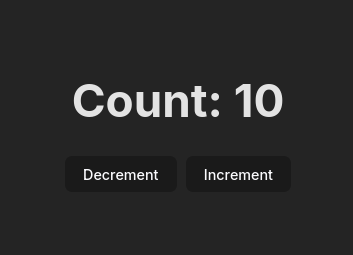
\includegraphics[width=0.7\textwidth]{useState-counter.png}}
    \caption{Counter using \texttt{useState()}}
    \end{figure}

    \section{Conclusion}
    This lab demonstrates the use of \texttt{useState()} in React to create a simple counter application. The \texttt{useState()} hook is used to manage the state of the counter, which is updated using the \texttt{setCount()} function. The \texttt{useState()} hook is a powerful tool for managing state in React applications.
    \\\\
    \vspace{1em}
    \begin{center}
        \rule{0.8\textwidth}{0.6pt}
    \end{center}
    \vspace{1em}

    \chapter{Computation of Circle Area using ReactJS}

    \section{Problem Statement}
    Implement a react app to calculate the area of a circle.

    \section{Computational Approach}
    Area of a circle is given by the formula:
    \[
        Area = \pi r^2
    \]
    \section{Implementation}
    Please note that the implementation of this practical uses the same CSS file as the previous practical.
    \begin{lstlisting}[caption={\texttt{App.jsx}}]
    import { useState } from "react"

    function App() {
      const [radius, setRadius] = useState("")
      const [area, setArea] = useState(null)

      const calculateArea = () => {
        const result = Math.PI * radius * radius
        setArea(result)
      }
      return (
        <div style={{ textAlign: "center", marginTop: "100px" }}>
          <h1>Area of a Circle</h1>

          <input
            type="number"
            placeholder="Enter radius"
            value={radius}
            onChange={(e) => setRadius(e.target.value)}
          />
          <br /><br />
          <button onClick={calculateArea}>
            Calculate
          </button>

          {area !== null && (
            <h2>Area: {area}</h2>
          )}
        </div>
      )
    }

    export default App
    \end{lstlisting}

    \section{Results}
    \begin{figure}[h]
        \centering
        \fbox{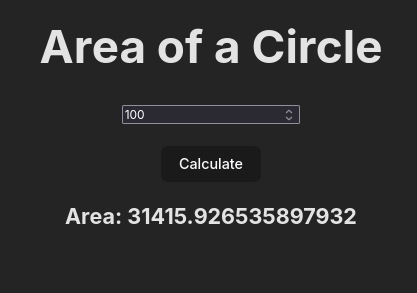
\includegraphics[width=0.7\textwidth]{circle-area.png}}
        \caption{React app that calculates circle area}
    \end{figure}
    \newpage

    \section{Conclusion}
    In this practical, we implemented a react app to calculate the area of a circle. We used the useState hook to manage the state of the radius and area. We also used the \texttt{Math.PI} constant to calculate the area of the circle.
    \\\\
        \vspace{1em}
        \begin{center}
            \rule{0.8\textwidth}{0.6pt}
        \end{center}
        \vspace{1em}

    \chapter{Form Validation and Controlled Components in ReactJS}

    \section{Problem Statement}
    Create a Sign-Up Form in React JS. The Sign-up form should ask for Name, Mobile, Email, Address, Date of Birth, Gender, Username, Password and Confirm Password. The Form should have two buttons, one for reset and one for submitting. The Submit Button should be enabled only when all the input values are validated.

    \section{Implementation}
    This practical uses React's \texttt{useState} hook to manage the state of form inputs such as name, mobile number, email, address, date of birth, gender, username, password, and confirm password. It also implements validation logic to ensure that all input fields satisfy the required constraints before enabling form submission. Conditional rendering and state updates are used to provide real-time feedback and control the disabled state of the submit button.
    Please note that the implementation of the this practical uses the same CSS file as the one used in Practical 04.

    \begin{lstlisting}[caption={\texttt{App.jsx}}]
    import './App.css'
    import { useState } from "react"

    function SignUp() {
      const [form, setForm] = useState({
        name: "",
        mobile: "",
        email: "",
        address: "",
        dob: "",
        gender: "",
        username: "",
        password: "",
        confirmPassword: ""
      })

      const handleChange = (e) => {
        setForm({ ...form, [e.target.name]: e.target.value })
      }

      const handleReset = () => {
        setForm({
          name: "",
          mobile: "",
          email: "",
          address: "",
          dob: "",
          gender: "",
          username: "",
          password: "",
          confirmPassword: ""
        })
      }

      const isValid =
        form.name &&
        form.mobile.length === 10 &&
        form.email.includes("@") &&
        form.address &&
        form.dob &&
        form.gender &&
        form.username &&
        form.password &&
        form.password === form.confirmPassword

      const handleSubmit = (e) => {
        e.preventDefault()
        alert("Form Submitted Successfully")
      }

      return (
        <div style={{ width: "400px", margin: "40px auto" }}>
          <h2>Sign-Up Form</h2>

          <form onSubmit={handleSubmit}>
            <input name="name" placeholder="Name" value={form.name} onChange={handleChange} /><br /><br />
            <input name="mobile" placeholder="Mobile" value={form.mobile} onChange={handleChange} /><br /><br />
            <input name="email" placeholder="Email" value={form.email} onChange={handleChange} /><br /><br />
            <input name="address" placeholder="Address" value={form.address} onChange={handleChange} /><br /><br />
            <input type="date" name="dob" value={form.dob} onChange={handleChange} /><br /><br />

            <select name="gender" value={form.gender} onChange={handleChange}>
              <option value="">Select Gender</option>
              <option value="Male">Male</option>
              <option value="Female">Female</option>
            </select><br /><br />

            <input name="username" placeholder="Username" value={form.username} onChange={handleChange} /><br /><br />
            <input type="password" name="password" placeholder="Password" value={form.password} onChange={handleChange} /><br /><br />
            <input type="password" name="confirmPassword" placeholder="Confirm Password" value={form.confirmPassword} onChange={handleChange} /><br /><br />

            <button type="reset" onClick={handleReset}>Reset</button>
            <button type="submit" disabled={!isValid} style={{ marginLeft: "10px" }}>
              Submit
            </button>
          </form>
        </div>
      )
    }

    export default SignUp
    \end{lstlisting}

    \section{Results}
    \begin{figure}[h]
    \centering
    \fbox{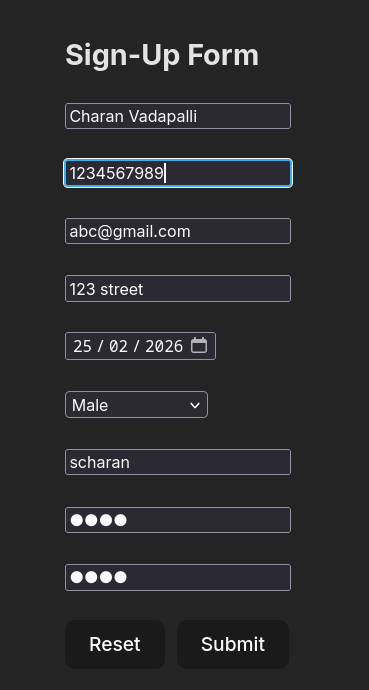
\includegraphics[height=0.3\textheight]{sign-up-form-react.png}}
    \caption{Sign-Up Form}
    \end{figure}
    \newpage

    \section{Conclusion}
    In this practical, a sign-up form was successfully implemented using React. The form includes fields for name, email, address, date of birth, gender, username, password, and confirm password. The form also includes validation to ensure that all fields are filled out correctly. The form was tested and found to be functional and user-friendly.
    \\\\
        \vspace{1em}
        \begin{center}
            \rule{0.8\textwidth}{0.6pt}
        \end{center}
        \vspace{1em}

    \chapter{Component Communication using Props in ReactJS}

    \section{Problem Statement}
    Implement a react app to pass the message ‘Hello from Parent’ from parent to child component using Props.

    \section{Theory}

    \subsection{Component-Based Architecture}
    React applications are crafted using several components that are reusable and independent. Each component encapsulates its own structure and logic.

    In a component hierarchy, a component that renders another component is called a parent component, and the rendered component is called a child component.

    \subsection{Data Flow in React}
    React follows a \textbf{unidirectional} data flow model. Data flows from parent to child components through props and a child cannot directly modify the parent's data. Communication from parent to child is achieved through props.
    \subsection{Props in React}
    \begin{definition}
        Props (properties) are read-only inputs passed from a parent component to a child component to configure its behavior and appearance.
    \end{definition}
    It's the immutable data that's passed to components as function parameters. The child component receives props as an object from the parent component and renders its UI based on the received props.

    In a component-based system, the parent generally owns the data or state and the child is only responsible for presentation. Therefore, props allow data sharing while maintaing separation of concerns. This ensures reusability, encapsulation, clear data ownership and predictable rendering behavior.

    \subsection{Parent to Child Communication}
    It occurs when:
    \begin{enumerate}
        \item The parent defines some data or state that the child component needs to render its UI.
        \item The parent passes that data or state to the child component as props.
        \item The child component needs to notify the parent about some event or state change.
        \item The child receives it as a parameter and renders its UI.
    \end{enumerate}
    This mechanism doesn't require state if the data doesn't change over time (dynamically).

    \section{Implementation}
    \begin{lstlisting}[caption={\texttt{App.jsx}}]
    function Child(props) {
      return (
        <div>
          <h1>This is the Child Component</h1>
          <h2>
            This is the message received: {props.message}
          </h2>
        </div>
      )
    }

    export default function Parent() {
      const dataToPass = "Hey there"

      return (
        <div>
          <h1>This is the Parent Component</h1>
          <br />
          <Child message={dataToPass} />
        </div>
      )
    }
    \end{lstlisting}
    \newpage

   \section{Results}
   \begin{figure}[h]
   \centering
   \fbox{
\includegraphics[width=0.8\textwidth]{parent-child-comp.png}}
   \caption{Demonstration of component communication}
   \end{figure}

   \section{Conclusion}
    In this implementation, data was successfully passed from a parent component to a child component using props. This demonstrates React’s unidirectional data flow model, where information flows from parent to child in a controlled and predictable manner. Props act as read-only inputs that allow components to communicate while maintaining separation of concerns. This approach promotes modular design, reusability, and clarity in component-based application development.
    \\\\
        \vspace{1em}
        \begin{center}
            \rule{0.8\textwidth}{0.6pt}
        \end{center}
        \vspace{1em}

\end{document}
